\documentclass[11pt,a4paper]{article}
\usepackage[T1]{fontenc}
\usepackage[utf8]{inputenc}
\usepackage{lmodern}
\usepackage{textcomp}
\usepackage[left=1.8cm,right=1.8cm,top=2.3cm,bottom=2.2cm,headheight=14pt,headsep=8pt]{geometry}
\usepackage{multicol}
\usepackage{xcolor}
\usepackage{fancyhdr}
\usepackage{graphicx}
\usepackage{array}
\usepackage{amsmath,amssymb}
\usepackage{setspace}
\usepackage{longtable}
\graphicspath{{../}}
\definecolor{ygreen}{RGB}{46,139,87}
\renewcommand{\normalsize}{\fontsize{10.9}{13.4}\selectfont}
\renewcommand{\familydefault}{\rmdefault}
\setlength{\parindent}{0pt}
\setlength{\columnsep}{0.8cm}
\setlength{\columnseprule}{0.4pt}
\setlength{\multicolsep}{3pt plus 1pt minus 1pt}
\renewcommand{\textsubscript}[1]{\ensuremath{_{\text{\fontsize{8}{8}\selectfont #1}}}}
\renewcommand{\textsuperscript}[1]{\ensuremath{^{\text{\fontsize{8}{8}\selectfont #1}}}}
\newcommand{\qn}[1]{\textbf{\fontsize{11.5}{13}\selectfont #1}}
\newcommand{\qsep}{\par\vspace{1pt}\noindent\rule{0pt}{0.4pt}\par\vspace{5pt}}
\newcommand{\fwrule}{\par\vspace{5pt}\noindent\rule{\linewidth}{1.4pt}\par\vspace{7pt}}
\newsavebox{\fitb}
\newcommand{\fitbox}[1]{\sbox{\fitb}{#1}\ifdim\wd\fitb>\linewidth\resizebox{\linewidth}{!}{\usebox{\fitb}}\else\usebox{\fitb}\fi}
\newcommand{\diqqat}[1]{\par\smallskip\noindent\textbf{Diqqat!} #1\par\medskip}
\newcommand{\javob}{\par\smallskip\noindent\textbf{Javob:} \rule[-2pt]{7.5cm}{0.4pt}\par\smallskip\noindent\textbf{Diqqat!} Javobingizni javoblar varaqasiga ko`chirib yozing.\par\medskip}
\pagestyle{fancy}
\fancyhf{}
\renewcommand{\headrulewidth}{0.4pt}
\fancyhead[L]{\textit{Milliy sertifikat 2026. Kimyo}}
\fancyhead[R]{6-variant}
\fancyfoot[L]{\fontsize{8}{9}\selectfont \textcopyright{} Colba maktabi, 2026}
\fancyfoot[C]{\thepage}
\fancypagestyle{first}{\fancyhf{}\renewcommand{\headrulewidth}{0pt}\fancyfoot[L]{\fontsize{8}{9}\selectfont \textcopyright{} Colba maktabi, 2026}\fancyfoot[C]{\thepage}}
\begin{document}
\normalsize
\thispagestyle{first}
\noindent\fcolorbox{ygreen}{white}{\parbox{\dimexpr\linewidth-2\fboxsep-2\fboxrule\relax}{%
\textbf{\fontsize{13}{15}\selectfont Nazorat testi}\ \textit{\fontsize{10}{12}\selectfont $\cdot$ Aralash test $\cdot$ 6-variant}\hfill
\begin{tabular}[t]{@{}r@{}}\textit{Milliy sertifikat 2026. Kimyo}\\ \textbf{\textit{\fontsize{8}{9}\selectfont Vaqt:}} \textit{\fontsize{10}{12}\selectfont 180 daqiqa}\end{tabular}}}
\par\medskip
\noindent\textit{Davriy jadvaldan foydalanish mumkin.}
\par\medskip
\begin{multicols}{2}
\noindent\qn{1.} Rasmda kristall panjara tuzilishi tasvirlangan.
\begin{center}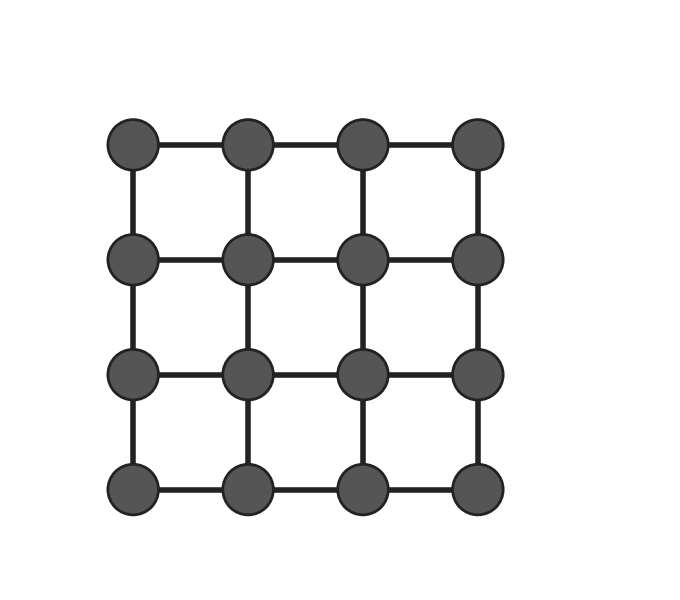
\includegraphics[width=0.86\linewidth]{rasmlar/gen/la_142898.png}\end{center}
Shunday panjarali moddalar uchun qaysi xususiyat xos?
\noindent A)~\textsl{Yuqori suyuqlanish harorati, suyuqlanmasi elektr tokini o`tkazadi}\par
\noindent B)~\textsl{Past suyuqlanish harorati, uchuvchan}\par
\noindent C)~\textsl{Juda qattiq, suyuqlanish harorati juda yuqori}\par
\noindent D)~\textsl{Elektr tokini yaxshi o`tkazadi, plastik}\par
\qsep
\noindent\qn{2.} 4 g metall oksidlanganda 5,6 g oksid hosil bo`ldi. Metallning ekvivalent \textbf{massasini (g/mol) aniqlang.}

\noindent A)~\textsl{40} \hfill B)~\textsl{20} \hfill C)~\textsl{10} \hfill D)~\textsl{30}\par
\qsep
\noindent\qn{3.} Radioaktiv izotop yadrolari sonining vaqtga bog`liqligi grafikda berilgan.
\begin{center}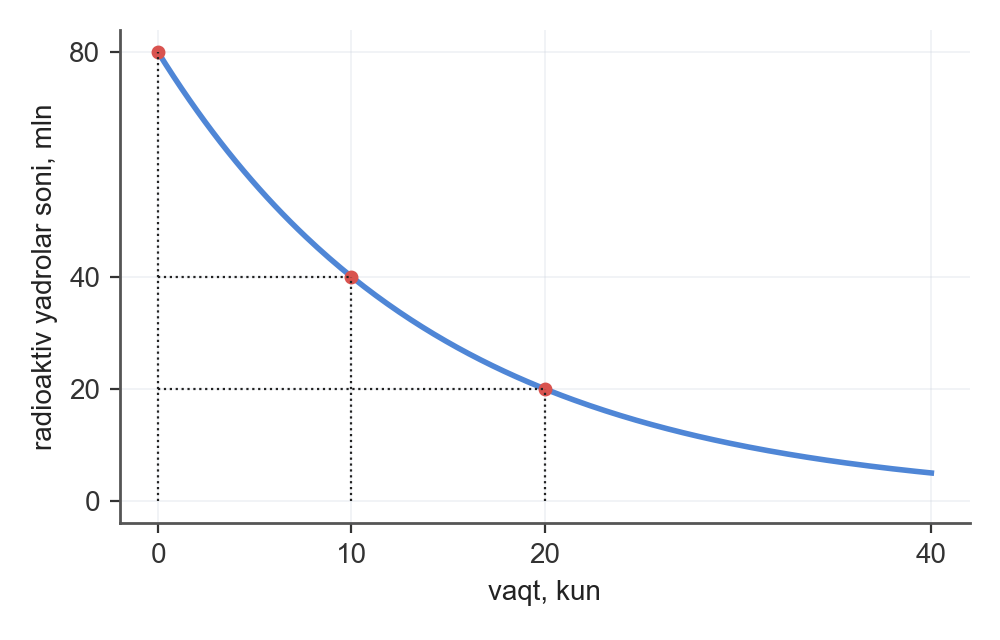
\includegraphics[width=0.86\linewidth]{rasmlar/gen/de_v06_0.png}\end{center}
20 kundan keyin necha mln yadro yemirilgan bo`ladi?

\noindent A)~\textsl{20} \hfill B)~\textsl{60} \hfill C)~\textsl{40} \hfill D)~\textsl{80}\par
\qsep
\noindent\qn{4.} C\textsubscript{6}H\textsubscript{5}CH\textsubscript{3} molekulasidagi $\sigma$ va $\pi$ bog`lar \textbf{sonini aniqlang.}

\noindent A)~\textsl{15 va 3} \hfill B)~\textsl{14 va 3} \hfill C)~\textsl{15 va 4} \hfill D)~\textsl{16 va 3}\par
\qsep
\noindent\qn{5.} Jadvalda Mn elementining birikmalaridagi oksidlanish darajasi berilgan:
\begin{center}
\renewcommand{\arraystretch}{1.15}
\fitbox{\begin{tabular}{|c|c|}\hline
\textbf{Modda} & \textbf{Oksidlanish darajasi} \\ \hline
K\textsubscript{2}MnO\textsubscript{4} & +6 \\ \hline
MnO\textsubscript{2} & +4 \\ \hline
KMnO\textsubscript{4} & +7 \\ \hline
MnSO\textsubscript{4} & +2 \\ \hline
\end{tabular}}
\end{center}
Ushbu moddalardan nechtasida Mn elementi ham oksidlovchi, ham qaytaruvchi xossani namoyon qiladi? (Mn uchun eng past oksidlanish darajasi 0, eng yuqorisi +7)

\noindent A)~\textsl{3} \hfill B)~\textsl{4} \hfill C)~\textsl{5} \hfill D)~\textsl{1}\par
\qsep
\noindent\qn{6.} Gazlar aralashmasi tarkibi jadvalda berilgan (n.sh.):
\begin{center}
\renewcommand{\arraystretch}{1.15}
\fitbox{\begin{tabular}{|c|c|}\hline
\textbf{Gaz} & \textbf{Hajmi, l} \\ \hline
H\textsubscript{2} & 3 \\ \hline
NH\textsubscript{3} & 2 \\ \hline
CH\textsubscript{4} & 3 \\ \hline
\end{tabular}}
\end{center}
Aralashmaning havoga nisbatan \textbf{zichligini aniqlang} (M(havo) = 29 g/mol).

\noindent A)~\textsl{0,76} \hfill B)~\textsl{0,19} \hfill C)~\textsl{0,38} \hfill D)~\textsl{11}\par
\qsep
\noindent\qn{7.} K\textsubscript{2}CO\textsubscript{3} ning suvli eritmasi inert elektrodlar bilan elektroliz qilinganda qaysi moddalar ajraladi?

\noindent\begin{tabular}{@{}p{0.47\linewidth}@{}p{0.47\linewidth}@{}}
A)~\textsl{Zn, H\textsubscript{2} va O\textsubscript{2}} & B)~\textsl{H\textsubscript{2} va O\textsubscript{2}} \\
C)~\textsl{Cu va Cl\textsubscript{2}} & D)~\textsl{Ag va O\textsubscript{2}} \\
\end{tabular}\par
\qsep
\noindent\qn{8.} S + HNO\textsubscript{3} $\to$ H\textsubscript{2}SO\textsubscript{4} + NO reaksiya tenglamasini tenglang va barcha koeffitsiyentlar \textbf{yig`indisini aniqlang.}

\noindent A)~\textsl{7} \hfill B)~\textsl{5} \hfill C)~\textsl{8} \hfill D)~\textsl{6}\par
\qsep
\noindent\qn{9.} Zn plastinka 33,1 g Pb(NO\textsubscript{3})\textsubscript{2} ni tutgan eritmaga tushirildi va Pb to`liq ajralib chiqquncha ushlab turildi. Plastinka massasi necha gramm ortadi?

\noindent A)~\textsl{28,4} \hfill B)~\textsl{7,1} \hfill C)~\textsl{33,1} \hfill D)~\textsl{14,2}\par
\qsep
\noindent\qn{10.} Massasi 7 g bo`lgan gaz 27 \textdegree{}C va 0,5 atm bosimda 12,3 l hajm egallaydi. Gazning vodorodga nisbatan \textbf{zichligini aniqlang.} (R = 0,082 l$\cdot$atm/(mol$\cdot$K))

\noindent A)~\textsl{14} \hfill B)~\textsl{28} \hfill C)~\textsl{7} \hfill D)~\textsl{56}\par
\qsep
\noindent\qn{11.} Quyidagi zarrachalardan qaysilari argon atomi bilan izoelektron? 1) Ca\textsuperscript{2+}; 2) K\textsuperscript{+}; 3) Cl\textsuperscript{$-$}; 4) Li\textsuperscript{+}

\noindent A)~\textsl{1, 2} \hfill B)~\textsl{1, 2, 3} \hfill C)~\textsl{1, 2, 4} \hfill D)~\textsl{1, 3}\par
\qsep
\noindent\qn{12.} 30-tartib raqamli element atomida n = 3 va l = 2 bo`lgan elektronlar \textbf{sonini aniqlang.}

\noindent A)~\textsl{11} \hfill B)~\textsl{10} \hfill C)~\textsl{9} \hfill D)~\textsl{12}\par
\qsep
\noindent\qn{13.} \textit{X} moddaning parchalanish reaksiyasida konsentratsiyaning vaqt bo`yicha o`zgarishi jadvalda berilgan:
\begin{center}
\renewcommand{\arraystretch}{1.15}
\fitbox{\begin{tabular}{|c|c|}\hline
\textbf{t, min} & \textbf{c, mol/l} \\ \hline
0 & 2,4 \\ \hline
2 & 1,92 \\ \hline
4 & 1,44 \\ \hline
6 & 0,96 \\ \hline
\end{tabular}}
\end{center}
0-minutdan 2-minutgacha o`rtacha tezlikni mol/(l$\cdot$min) \textbf{hisoblang.}

\noindent A)~\textsl{0,48} \hfill B)~\textsl{0,12} \hfill C)~\textsl{1,2} \hfill D)~\textsl{0,24}\par
\qsep
\noindent\qn{14.} Qaysi juftliklar o`zaro reaksiyaga kirishadi? 1) SiO\textsubscript{2} va H\textsubscript{2}O; 2) Ag va H\textsubscript{2}SO\textsubscript{4}(suyult.); 3) MgCl\textsubscript{2} va KNO\textsubscript{3}; 4) Fe va HCl

\noindent A)~\textsl{2, 3} \hfill B)~\textsl{1} \hfill C)~\textsl{3, 4} \hfill D)~\textsl{4}\par
\qsep
\noindent\qn{15.} 37,8 g Zn(NO\textsubscript{3})\textsubscript{2} to`liq parchalanguncha qizdirildi. Qattiq qoldiq \textbf{massasini (g) aniqlang.}

\noindent A)~\textsl{16,2} \hfill B)~\textsl{37,8} \hfill C)~\textsl{32,4} \hfill D)~\textsl{8,1}\par
\qsep
\noindent\qn{16.} 0,2 mol NaOH tutgan eritmadan 0,15 mol CO\textsubscript{2} o`tkazildi. Hosil bo`lgan NaHCO\textsubscript{3} \textbf{massasini (g) aniqlang.}

\noindent A)~\textsl{8,4} \hfill B)~\textsl{4,2} \hfill C)~\textsl{2,1} \hfill D)~\textsl{8}\par
\qsep
\noindent\qn{17.} Reaksiya tenglamasi: 2NaCl + H\textsubscript{2}SO\textsubscript{4} $\to$ Na\textsubscript{2}SO\textsubscript{4} + 2HCl. Reaksiyaga 196 g H\textsubscript{2}SO\textsubscript{4} kirishdi. HCl \textbf{massasini (g) hisoblang.}

\noindent A)~\textsl{36,5} \hfill B)~\textsl{292} \hfill C)~\textsl{146} \hfill D)~\textsl{73}\par
\qsep
\noindent\qn{18.} Li va K dan iborat 6 g aralashma suv bilan reaksiyaga kirishdi. Ajralgan vodorodning \textbf{hajmini (l, n.sh.) aniqlang.}

\noindent A)~\textsl{4,48} \hfill B)~\textsl{8,96} \hfill C)~\textsl{2,24} \hfill D)~\textsl{3}\par
\qsep
\noindent\qn{19.} Alyuminiy (0,2 mol) va magniy (0,2 mol) aralashmasi mo`l xlorid kislotada eritildi. Ajralgan vodorodning \textbf{hajmini (l, n.sh.) aniqlang.}

\noindent A)~\textsl{11,2} \hfill B)~\textsl{8,96} \hfill C)~\textsl{22,4} \hfill D)~\textsl{5,6}\par
\qsep
\noindent\qn{20.} CH\textsubscript{3}--CH(CH\textsubscript{3})--CH(C\textsubscript{2}H\textsubscript{5})--CH\textsubscript{2}--CH\textsubscript{3} birikmaning sistematik nomi qaysi qatorda to`g`ri keltirilgan?

\noindent\begin{tabular}{@{}p{0.47\linewidth}@{}p{0.47\linewidth}@{}}
A)~\textsl{2-metil-3-etilpentan} & B)~\textsl{3-izopropilpentan} \\
C)~\textsl{3-etil-2-metilpentan} & D)~\textsl{2,3-dietilbutan} \\
\end{tabular}\par
\qsep
\noindent\qn{21.} Alken, alkadiyen va alkinlar haqida qaysi fikrlar to`g`ri? 1) Asetilen Ag\textsubscript{2}O ning ammiakli eritmasi bilan cho`kma beradi (butin-2 beradi); 2) Etilen sanoatda kreking gazlaridan olinadi; 3) Alkinlar uchun umumiy formula CnH\textsubscript{2}n+2; 4) Kauchuk izoprenning polimeri

\noindent A)~\textsl{1, 3} \hfill B)~\textsl{1, 4} \hfill C)~\textsl{2, 4} \hfill D)~\textsl{1, 3, 4}\par
\qsep
\noindent\qn{22.} 18,8 g fenoldan 2,4,6-tribromfenol olishda unum 75\% bo`lsa, mahsulot \textbf{massasini (g) aniqlang.}

\noindent A)~\textsl{66,2} \hfill B)~\textsl{99,3} \hfill C)~\textsl{14,1} \hfill D)~\textsl{49,65}\par
\qsep
\noindent\qn{23.} C\textsubscript{6}H\textsubscript{5}OH + 3Br\textsubscript{2} $\to$ C\textsubscript{6}H\textsubscript{2}Br\textsubscript{3}OH + 3HBr reaksiyasida 9,4 g C\textsubscript{6}H\textsubscript{5}OH ishtirok etdi. C\textsubscript{6}H\textsubscript{2}Br\textsubscript{3}OH \textbf{miqdorini (mol) toping.}

\noindent A)~\textsl{0,1} \hfill B)~\textsl{0,2} \hfill C)~\textsl{0,05} \hfill D)~\textsl{0,15}\par
\qsep
\noindent\qn{24.} 11,6 g propanal Ag\textsubscript{2}O ning ammiakli eritmasi bilan to`liq oksidlanganda hosil bo`lgan kumush \textbf{massasini (g) aniqlang.}

\noindent A)~\textsl{21,6} \hfill B)~\textsl{43,2} \hfill C)~\textsl{86,4} \hfill D)~\textsl{11,6}\par
\qsep
\noindent\qn{25.} 60 g CH\textsubscript{3}COOH dan quyidagi ikki bosqichda Na\textsubscript{2}CO\textsubscript{3} olinadi: 1) CH\textsubscript{3}COOH + NaOH $\to$ CH\textsubscript{3}COONa + H\textsubscript{2}O (unum 90\%); 2) CH\textsubscript{3}COONa + NaOH $\to$ CH\textsubscript{4} + Na\textsubscript{2}CO\textsubscript{3} (unum 50\%). Oxirgi mahsulot Na\textsubscript{2}CO\textsubscript{3} ning \textbf{massasini (g) toping.}

\noindent A)~\textsl{53} \hfill B)~\textsl{95,4} \hfill C)~\textsl{47,7} \hfill D)~\textsl{106}\par
\qsep
\noindent\qn{26.} 60 g CH\textsubscript{3}COOH dan quyidagi ikki bosqichda CH\textsubscript{3}COONa olinadi: 1) CH\textsubscript{3}COOH + C\textsubscript{2}H\textsubscript{5}OH $\to$ CH\textsubscript{3}COOC\textsubscript{2}H\textsubscript{5} + H\textsubscript{2}O (unum 60\%); 2) CH\textsubscript{3}COOC\textsubscript{2}H\textsubscript{5} + NaOH $\to$ CH\textsubscript{3}COONa + C\textsubscript{2}H\textsubscript{5}OH (unum 50\%). Oxirgi mahsulot CH\textsubscript{3}COONa ning \textbf{massasini (g) toping.}

\noindent A)~\textsl{41} \hfill B)~\textsl{24,6} \hfill C)~\textsl{49,2} \hfill D)~\textsl{82}\par
\qsep
\noindent\qn{27.} Uglevodlar haqida qaysi fikrlar to`g`ri? 1) Kraxmal va selluloza bir xil M ga ega; 2) Saxaroza Feling suyuqligini qaytaradi; 3) Maltoza gidrolizlanganda ikki molekula glyukoza hosil qiladi; 4) Glyukoza "kumush ko`zgu" reaksiyasini beradi

\noindent A)~\textsl{3, 4} \hfill B)~\textsl{1, 3} \hfill C)~\textsl{2} \hfill D)~\textsl{2, 3}\par
\qsep
\noindent\qn{28.} Quyidagi birikmalardan qaysi biri fenol sinfiga kiradi?

\noindent\begin{tabular}{@{}p{0.47\linewidth}@{}p{0.47\linewidth}@{}}
A)~\textsl{H\textsubscript{2}NCH\textsubscript{2}COOH} & B)~\textsl{CH\textsubscript{3}CHO} \\
C)~\textsl{C\textsubscript{6}H\textsubscript{12}O\textsubscript{6}} & D)~\textsl{C\textsubscript{6}H\textsubscript{5}OH} \\
\end{tabular}\par
\qsep
\noindent\qn{29.} Izobutilen monomeridan olingan polimerning molyar massasi 140000 g/mol. Polimerlanish \textbf{darajasini aniqlang.}

\noindent A)~\textsl{5000} \hfill B)~\textsl{1250} \hfill C)~\textsl{2500} \hfill D)~\textsl{2510}\par
\qsep
\noindent\qn{30.} Rasmdagi tajribada etanolga konsentrlangan H\textsubscript{2}SO\textsubscript{4} ning vazifasi nima?
\begin{center}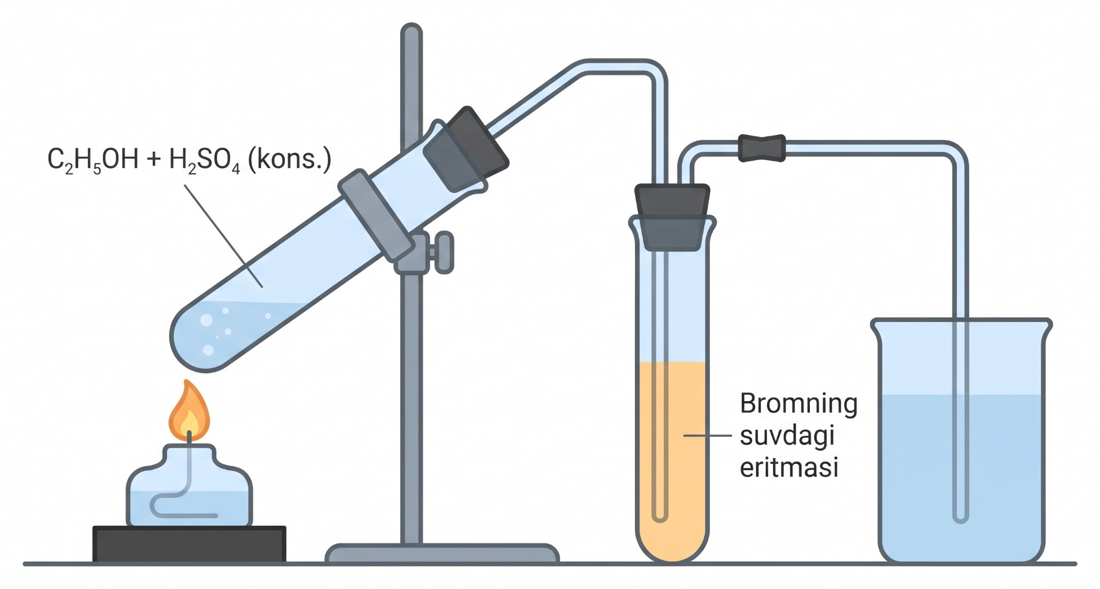
\includegraphics[width=0.86\linewidth]{rasmlar/darslik/d_etilen.png}\end{center}
\noindent A)~\textsl{oksidlovchi, etilenni oksidlaydi}\par
\noindent B)~\textsl{faqat erituvchi}\par
\noindent C)~\textsl{reaksiyada ishtirok etmaydi}\par
\noindent D)~\textsl{suv tortuvchi va katalizator}\par
\qsep
\noindent\qn{31.} Kimyo laboratoriyasida ishlash qoidalari haqida qaysi fikrlar to`g`ri? 1) Zaharli gaz ajraladigan tajriba mo`rili shkafda o`tkaziladi; 2) Kimyoviy moddalar hidini bevosita nafas olib aniqlash kerak; 3) Suvni konsentrlangan kislotaga tez quyish mumkin; 4) Ortiqcha reaktiv idishga qaytariladi

\noindent A)~\textsl{1, 4} \hfill B)~\textsl{1, 3} \hfill C)~\textsl{1} \hfill D)~\textsl{4}\par
\qsep
\noindent\qn{32.} 400 g 4\% li CuSO\textsubscript{4} eritmasini CuSO\textsubscript{4}$\cdot$5H\textsubscript{2}O dan tayyorlash uchun necha gramm kristallogidrat kerak?

\noindent A)~\textsl{16} \hfill B)~\textsl{50} \hfill C)~\textsl{12,5} \hfill D)~\textsl{25   ---}\par
\qsep
\end{multicols}
\medskip
\noindent\setlength{\fboxsep}{0pt}\fbox{\begin{tabular}{p{0.74\linewidth}|p{0.2\linewidth}}
\parbox[t]{0.72\linewidth}{\vspace{3pt}\textbf{Topshiriqlar (33--35) va javob variant (A--F)larini o`zaro to`g`ri moslashtiring.} CuO va Fe\textsubscript{2}O\textsubscript{3} dan iborat 32 g aralashma qizdirilib, H\textsubscript{2} oqimida to`liq qaytarildi; qoldiq (metallar) massasi 24 g.
\vspace{3pt}} & \parbox[t]{0.19\linewidth}{\vspace{3pt}A~\textsl{18}\\[3pt]
B~\textsl{9}\\[3pt]
C~\textsl{16}\\[3pt]
D~\textsl{13,44}\\[3pt]
E~\textsl{12,8}\\[3pt]
F~\textsl{24}}\\ \hline
\parbox[t]{0.72\linewidth}{\vspace{2pt}\textbf{33. Aralashmadagi CuO massasini (g) aniqlang.}\vspace{2pt}} & \\ \hline
\parbox[t]{0.72\linewidth}{\vspace{2pt}\textbf{34. Qaytarish uchun (20\% ortiqcha olingan) sarflangan H\textsubscript{2} hajmini (l, n.sh.) aniqlang.}\vspace{2pt}} & \\ \hline
\parbox[t]{0.72\linewidth}{\vspace{2pt}\textbf{35. Qaytarish natijasida hosil bo`lgan suv massasini (g) aniqlang.}\vspace{2pt}} & 
\end{tabular}}
\par\bigskip
\noindent\qn{36.} KMnO\textsubscript{4} + Na\textsubscript{2}SO\textsubscript{3} + H\textsubscript{2}O $\to$ MnO\textsubscript{2} + Na\textsubscript{2}SO\textsubscript{4} + KOH reaksiya tenglamasini tenglang. Reagentlar (chap qism) koeffitsiyentlari \textbf{yig`indisini toping.}
\javob\qsep
\noindent\qn{37.} NaCl eritmasi inert elektrodlar yordamida 2 A tok kuchi bilan 3860 s elektroliz qilindi. Katodda ajralgan H\textsubscript{2} massasi (g) \textbf{ni toping.}
\javob\qsep
\noindent\qn{38.} Zn va ZnO dan iborat 22,7 g aralashma mo`l NaOH eritmasida eritilganda 2,24 l (n.sh.) vodorod ajraldi. Aralashmadagi ZnO \textbf{massasini (g) aniqlang.}
\javob\qsep
\noindent\qn{39.} Etanol va fenoldan iborat 23,4 g aralashma natriy bilan to`liq reaksiyaga kirishganda 3,36 l (n.sh.) vodorod ajraldi. Shu aralashmaga mo`l bromli suv ta'sir ettirilganda hosil bo`ladigan cho`kma \textbf{massasini (g) toping.}
\javob\qsep
\noindent\qn{40.} Etilen monomeridan olingan polimerning molyar massasi 56000 g/mol. Polimerlanish \textbf{darajasini aniqlang.}
\javob\qsep
\par\bigskip\begin{center}\textbf{\fontsize{13}{15}\selectfont YOZMA ISH}\end{center}
\noindent\qn{41.} \textbf{Topshiriqni bajarish jarayonida barcha reaksiya tenglamalarini yozing. Miqdoriy va arifmetik hisoblashlarni (unga asos bo`lgan usul yoki formulani ko`rsatgan holda) uzviy ketma-ketlikda bajaring.}\par\smallskip
300 g 20\% li NaCl eritmasi inert elektrodlar yordamida 5 A tok kuchi bilan 3860 s elektroliz qilindi.\par
\noindent 1)Katodda va anodda ajralgan gazlarning hajmlarini (l, n.sh.) hisoblang.\par
\noindent 2)Elektrolizdan keyingi eritma massasini (g) aniqlang. Ajralgan gazlarning umumiy massasini (g) ham hisoblang.\par
\noindent 3)Elektrolizdan keyingi eritmada NaOH ning massa ulushini (\%) toping.\par
\noindent 4)Hosil bo`lgan NaOH ni to`liq neytrallash uchun 10\% li HCl eritmasidan necha gramm kerak? Hosil bo`lgan NaCl massasini (g) ham hisoblang.\par
\noindent 5)Anodda ajralgan xlor KI eritmasidan o`tkazilsa, ajralgan yod massasini (g) aniqlang. Anodda ajralgan xlorning massasini (g) ham toping.\par
\diqqat{Mazkur topshiriq kengaytirilgan javobni talab etib, uning yechilish usuli va shu usul asosidagi barcha hisoblash amallari javoblar varaqasida aks etishi lozim.}\qsep
\noindent\qn{42.} Reaksiya tenglamalarini tugallang va tenglang. Hosil bo`lgan organik moddalarning tuzilish formulalarini yozing va ularni nomlang.\par
\noindent 1)C\textsubscript{6}H\textsubscript{5}--CH\textsubscript{3} + Cl\textsubscript{2} $\xrightarrow{\text{yorug`lik}}$\par
\noindent 2)CH\textsubscript{3}--CH\textsubscript{2}--OH + CuO $\xrightarrow{\text{t}}$\par
\noindent 3)2CH\textsubscript{4} $\xrightarrow{\text{1500 \textdegree{}C}}$\par
\noindent 4)CH\textsubscript{3}CHO + Ag\textsubscript{2}O $\xrightarrow{\text{NH\textsubscript{3}, t}}$\par
\noindent 5)C\textsubscript{2}H\textsubscript{5}Br + KOH(spirtli) $\to$\par
\noindent 6)n CH\textsubscript{2}=CH--CH=CH\textsubscript{2} $\to$\par
\noindent 7)CH\textsubscript{3}--CH=CH\textsubscript{2} + HBr $\to$\par
\diqqat{Mazkur topshiriq kengaytirilgan javobni talab etib, uning yechilish usuli va shu usul asosidagi barcha hisoblash amallari javoblar varaqasida aks etishi lozim.}\qsep
\noindent\qn{43.} \textbf{Topshiriqni bajarish jarayonida barcha reaksiya tenglamalarini yozing. Miqdoriy va arifmetik hisoblashlarni (unga asos bo`lgan usul yoki formulani ko`rsatgan holda) uzviy ketma-ketlikda bajaring.}\par\smallskip
0,05 mol AlCl\textsubscript{3} saqlagan eritmaga NaOH eritmasi qo`shildi. Avval 0,15 mol NaOH qo`shilganda cho`kma hosil bo`ldi, so`ng yana 0,05 mol NaOH qo`shilganda cho`kma to`liq erib ketdi (Na[Al(OH)\textsubscript{4}] hosil bo`ldi).\par
\noindent 1)Cho`kma hosil bo`lish va erish reaksiyalari tenglamalarini yozing. Cho`kma massasini (g) hisoblang.\par
\noindent 2)Jami sarflangan NaOH massasini (g) aniqlang.\par
\noindent 3)Hosil bo`lgan Na[Al(OH)\textsubscript{4}] eritmasidan mo`l CO\textsubscript{2} o`tkazilganda cho`kadigan Al(OH)\textsubscript{3} massasini (g) toping.\par
\noindent 4)Al(OH)\textsubscript{3} cho`kmasi qizdirilganda hosil bo`ladigan oksid massasini (g) hisoblang.\par
\noindent 5)Na[Al(OH)\textsubscript{4}] eritmasining hajmi 500 ml bo`lsa, tuzning molyar konsentratsiyasini (mol/l) hisoblang.\par
\diqqat{Mazkur topshiriq kengaytirilgan javobni talab etib, uning yechilish usuli va shu usul asosidagi barcha hisoblash amallari javoblar varaqasida aks etishi lozim.}\qsep
\newpage
\noindent\textbf{\fontsize{13}{15}\selectfont Nazorat testi}\ \textit{$\cdot$ 6-variant}\hfill \textbf{Javoblar kaliti}\par\smallskip\hrule\smallskip
\textit{Faqat o`qituvchi uchun.}\par\medskip
\noindent\textbf{1--32-savollar}\par\smallskip
\noindent\begin{tabular}{|c|c|c|c|c|c|c|c|c|c|c|c|c|c|c|c|}\hline
\textbf{1} & \textbf{2} & \textbf{3} & \textbf{4} & \textbf{5} & \textbf{6} & \textbf{7} & \textbf{8} & \textbf{9} & \textbf{10} & \textbf{11} & \textbf{12} & \textbf{13} & \textbf{14} & \textbf{15} & \textbf{16}\\\hline
\textsl{C} & \textsl{B} & \textsl{B} & \textsl{A} & \textsl{A} & \textsl{C} & \textsl{B} & \textsl{D} & \textsl{D} & \textsl{A} & \textsl{B} & \textsl{B} & \textsl{D} & \textsl{D} & \textsl{A} & \textsl{B}\\\hline
\textbf{17} & \textbf{18} & \textbf{19} & \textbf{20} & \textbf{21} & \textbf{22} & \textbf{23} & \textbf{24} & \textbf{25} & \textbf{26} & \textbf{27} & \textbf{28} & \textbf{29} & \textbf{30} & \textbf{31} & \textbf{32}\\\hline
\textsl{C} & \textsl{A} & \textsl{A} & \textsl{C} & \textsl{C} & \textsl{D} & \textsl{A} & \textsl{B} & \textsl{C} & \textsl{B} & \textsl{A} & \textsl{D} & \textsl{C} & \textsl{D} & \textsl{C} & \textsl{D}\\\hline
\end{tabular}\par\medskip
\noindent\textbf{33--35-savollar}\par\smallskip
\noindent\begin{tabular}{|c|c|c|}\hline \textbf{No} & \textbf{Javob} & \textbf{Qiymat}\\\hline
33 & \textsl{C} & 16\\\hline
34 & \textsl{D} & 13,44\\\hline
35 & \textsl{B} & 9\\\hline
\end{tabular}\par\medskip
\noindent\textbf{36--40-savollar}\par\smallskip
\noindent\begin{tabular}{|c|c|}\hline \textbf{No} & \textbf{To`g`ri javob}\\\hline
36 & 6\\\hline
37 & 0,08\\\hline
38 & 16,2\\\hline
39 & 66,2\\\hline
40 & 2000\\\hline
\end{tabular}\par\medskip
\noindent\textbf{41--43-topshiriqlar: javoblar}\par\smallskip
\noindent\textbf{41-topshiriq.}\par
\noindent 1) 2,24 l; 2,24 l\par
\noindent 2) 292,7 g; 7,3 g\par
\noindent 3) 2,73\%\par
\noindent 4) 73 g; 11,7 g\par
\noindent 5) 25,4 g; 7,1 g\par
\noindent\textbf{42-topshiriq.}\par
\noindent 1) C\textsubscript{6}H\textsubscript{5}--CH\textsubscript{3} + Cl\textsubscript{2} $\xrightarrow{\text{yorug`lik}}$ C\textsubscript{6}H\textsubscript{5}CH\textsubscript{2}Cl + HCl --- benzilxlorid (4 ball)\par
\noindent 2) CH\textsubscript{3}--CH\textsubscript{2}--OH + CuO $\xrightarrow{\text{t}}$ CH\textsubscript{3}CHO + Cu + H\textsubscript{2}O --- etanal (3 ball)\par
\noindent 3) 2CH\textsubscript{4} $\xrightarrow{\text{1500 \textdegree{}C}}$ C\textsubscript{2}H\textsubscript{2} + 3H\textsubscript{2} --- asetilen (3 ball)\par
\noindent 4) CH\textsubscript{3}CHO + Ag\textsubscript{2}O $\xrightarrow{\text{NH\textsubscript{3}, t}}$ CH\textsubscript{3}COOH + 2Ag$\downarrow$ --- etan (sirka) kislota (4 ball)\par
\noindent 5) C\textsubscript{2}H\textsubscript{5}Br + KOH(spirtli) $\to$ CH\textsubscript{2}=CH\textsubscript{2} + KBr + H\textsubscript{2}O --- etilen (3 ball)\par
\noindent 6) n CH\textsubscript{2}=CH--CH=CH\textsubscript{2} $\to$ (--CH\textsubscript{2}--CH=CH--CH\textsubscript{2}--)n --- polibutadiyen (4 ball)\par
\noindent 7) CH\textsubscript{3}--CH=CH\textsubscript{2} + HBr $\to$ CH\textsubscript{3}--CHBr--CH\textsubscript{3} --- 2-brompropan (Markovnikov) (4 ball)\par
\noindent\textbf{43-topshiriq.}\par
\noindent 1) 3,9 g\par
\noindent 2) 8 g\par
\noindent 3) 3,9 g\par
\noindent 4) 2,55 g\par
\noindent 5) 0,1 mol/l\par
\par\bigskip\noindent\textbf{Mavzular taqsimoti}\par\smallskip
{\small\noindent\begin{longtable}{|c|p{7.2cm}|p{5.4cm}|c|}\hline \textbf{No} & \textbf{Mavzu} & \textbf{Tekshiriladigan ko`nikma} & \textbf{Ball}\\\hline
1 & 8-sinf (kristall panjaralar) & Rasm bo`yicha tahlil & 1\\\hline
2 & 11-sinf (ekvivalentlar qonuni) & Hisoblash va masala yechish & 1\\\hline
3 & 11-sinf (yadro) & Grafik tahlili & 1\\\hline
4 & 10-sinf \S{}17 (gibridlanish); Abdusamatov & Bilim va tushunish & 1\\\hline
5 & Tirkashev \textit{V} bob (OQR, jadval) & Jadval tahlili & 1\\\hline
6 & 11-sinf (gaz aralashmalar, jadval) & Jadval tahlili & 1\\\hline
7 & 11-sinf 8-bob; Tirkashev \textit{V} bob (elektroliz) & Bilim va tushunish & 1\\\hline
8 & Tirkashev \textit{V} bob; 11-sinf 7-bob (OQR tenglash) & Hisoblash va masala yechish & 1\\\hline
9 & Tashev; 9-sinf (metallarning kuchlanish qatori) & Hisoblash va masala yechish & 1\\\hline
10 & 11-sinf (Mendeleyev--Klapeyron) & Hisoblash va masala yechish & 1\\\hline
11 & Tirkashev I bob; 8-sinf (izoelektron) & Bilim va tushunish & 1\\\hline
12 & Tirkashev I bob; 8-sinf (elektron konfiguratsiya) & Bilim va tushunish & 1\\\hline
13 & Tirkashev VI bob (tezlik, jadval) & Jadval tahlili & 1\\\hline
14 & 9-sinf; Tashev (anorganik birikmalar xossalari) & Bilim va tushunish & 1\\\hline
15 & Tashev (nitratlar termik parchalanishi) & Hisoblash va masala yechish & 1\\\hline
16 & 9-sinf (uglerod (IV) oksid) & Hisoblash va masala yechish & 1\\\hline
17 & 9-sinf; Tirkashev (galogenlar, hisob) & Hisoblash va masala yechish & 1\\\hline
18 & 9-sinf (ishqoriy metallar) & Hisoblash va masala yechish & 1\\\hline
19 & 9-sinf & Hisoblash va masala yechish & 1\\\hline
20 & 10-sinf (nomenklatura \S{}6, \S{}11, \S{}20, \S{}24--26) & Bilim va tushunish & 1\\\hline
21 & 10-sinf (mavzuga oid paragraflar); Abdusamatov & Bilim va tushunish & 1\\\hline
22 & 10-sinf \S{}16, \S{}23, \S{}33 & Hisoblash va masala yechish & 1\\\hline
23 & 10-sinf (spirt, hisob) & Hisoblash va masala yechish & 1\\\hline
24 & 10-sinf \S{}24; \S{}26; \S{}30 (kumush ko`zgu) & Hisoblash va masala yechish & 1\\\hline
25 & 10-sinf (ikki bosqichli hisob) & Hisoblash va masala yechish & 1\\\hline
26 & 10-sinf (ikki bosqichli hisob) & Hisoblash va masala yechish & 1\\\hline
27 & 10-sinf (mavzuga oid paragraflar); Abdusamatov & Bilim va tushunish & 1\\\hline
28 & 10-sinf (organik birikmalar sinflari) & Bilim va tushunish & 1\\\hline
29 & 10-sinf \S{}35 & Hisoblash va masala yechish & 1\\\hline
30 & 10-sinf (6-rasm) & Rasm bo`yicha tahlil & 1\\\hline
31 & 7-sinf (xavfsizlik qoidalari); 10-sinf lab. & Bilim va tushunish & 1\\\hline
32 & Tirkashev III bob; 7-sinf (eritma tayyorlash) & Hisoblash va masala yechish & 1\\\hline
33--35 & Aralash masala (moslashtirish) & Ko`p bosqichli hisob & 3\\\hline
36--40 & Qisqa javobli masalalar & Hisoblash & 5\\\hline
41--43 & Yozma ish & Usul va hisob (M, A) & 75\\\hline
\end{longtable}}
\end{document}
